\documentclass[11pt]{article}
\usepackage[utf8]{inputenc}
\usepackage[T1]{fontenc}
\usepackage{lmodern}
\usepackage[french]{babel}
\usepackage{amsmath, amsthm, epsfig, amsfonts, amssymb, listings, enumerate,
color, hyperref, mdframed}

\usepackage{fancyhdr}
\usepackage{lastpage}

\pagestyle{fancy}
\lhead{Programmation en C}
\chead{}
\rhead{EPFL -- Automne 2017}
\headsep = 24pt
\fancyfoot{}
\rfoot{\thepage\ / \pageref{LastPage}}
\renewcommand{\headrule}{\vbox to 0pt{\hbox to \headwidth{\dotfill}\vss}}
\fancyhfoffset[H]{0pt}
\renewcommand{\footrulewidth}{0pt}

\definecolor{dkgreen}{rgb}{0,0.6,0}
\definecolor{gray}{rgb}{0.5,0.5,0.5}
\definecolor{mauve}{rgb}{0.58,0,0.82}

\definecolor{mygray}{rgb}{0.4,0.4,0.4}
\definecolor{mygreen}{rgb}{0,0.8,0.6}
\definecolor{myorange}{rgb}{1.0,0.4,0}
\lstset{frame=tblr,
  language=[ANSI]C,
  aboveskip=3mm,
  belowskip=3mm,
  showstringspaces=false,
  columns=flexible,
  basicstyle={\small\ttfamily},
%  numbers=left,
  numberstyle=\tiny\color{gray},
  keywordstyle=\color{blue},
  commentstyle=\color{dkgreen},
  stringstyle=\color{mauve},
  breaklines=true,
  breakatwhitespace=true
  tabsize=3
}

\textheight 23cm
\textwidth 16.5cm
\voffset -2.5cm
\hoffset -2cm

\parindent 0cm
\parskip.5\baselineskip

\begin{document}

%========================
\begin{center}{\bf Session d'exercices -- Pointeurs}\\
\textbf{\emph{Moyenne glissante}}
\end{center}
En traitement du signal, on sait qu'un signal échantilloné a une certaine fréquence d'échantillonage peut être parfaitement reconstruit si la fréquence du signal est strictement inférieure à la moitié de la fréquence d'échantillonage. On appelle cette fréquence maximale la fréquence de Nyquist. Dans cet exercice, nous définirons deux structures représentant les caractéristiques d'un signal sinusoïdal simple et d'un échantillonage et utiliserons ensuite ces structures pour vérifier la théorie en échantillonant des signaux de fréquences diverses. A noter que dans cet exercice, un signal complet est défini comme étant une somme de signaux sinusoïdaux.\\
\\
Si la théorie sous-jacente n'est plus très claire pour vous, vous trouverez des informations sur les pages suivantes : 
\begin{enumerate}
\item Signaux sinusoïdes % : $https://fr.wikipedia.org/wiki/Signal_sinuso%C3%AFdal$
\item Echantillonage :% $https://fr.wikipedia.org/wiki/%C3%89chantillonnage_(signal)$
\item Théorème d'échantillonage : %$https://fr.wikipedia.org/wiki/Th%C3%A9or%C3%A8me_d%27%C3%A9chantillonnage$
\end{enumerate}




\newpage
\begin{enumerate}[a)]


\item \textcolor{mygreen}{[Difficulté: *]}
Ecrivez la structure
\begin{center}
\texttt{Sinusoide}, 
\end{center}
qui doit contenir 3 champs représentant les 3 constantes inhérentes d'un signal sinusoïdal pur : la fréquence, l'amplitude et le déphasage.

\item \textcolor{mygreen}{[Difficulté: *]}
Écrivez la structure
\begin{center} 
\texttt{Echantillonage}, 
\end{center}
qui doit contenir 2 champs représentant l'instant auquel l'échantillonage commence et sa fréquence.

\vspace{20pt}
\hspace{-20pt} Continuez en écrivant tout ce qui manque pour compléter le programme, incluant ce qui suit :
\vspace{20pt}

\item \textcolor{mygreen}{[Difficulté: **]}
Écrivez la fonction
\begin{center} 
%\texttt{double sin_pure(double t, struct Sinusoide s)}, 
\texttt{double movAvg(float *in, float *out, int m)}, 
\end{center}
qui prend en argument un réel et une structure Sinusoïde et retourne la valeur de la sinusoïde à un instant t. Si l'utilisation des 3 constantes d'une sinusoïde n'est pas claire, se référer aux pages de théorie plus haut.

\vspace{20pt}


\item \textcolor{mygreen}{[Difficulté: **]}
Écrivez la fonction 

\begin{center}
\texttt{void movAvg(float *in, float *out, int m)}, 
\end{center}

qui prend comme arguments les adresses de début du tableau de données et du tableau contenant les moyennes, ainsi que la taille du groupe d'éléments utilisés pour calculer chaque moyenne. Cette fonction remplit le tableau des moyennes suivant le premier exemple (simple moving average) et affiche tous les éléments de ce tableau comme dans l'exemple de sortie au bas de cette page.

\item \textcolor{mygreen}{[Difficulté: ***]}
Écrivez la fonction

\begin{center} 
\texttt{void movAvgFull(float *in, float *out, int m)}, 
\end{center}

qui prend comme arguments les adresses de début du tableau de données et du tableau contenant les moyennes, ainsi que la taille du groupe d'éléments utilisés pour calculer chaque moyenne. Cette fonction remplit le tableau des moyennes suivant le deuxième exemple (full moving average) et affiche tous les éléments de ce tableau comme dans l'exemple de sortie au bas de cette page.

\vspace{20pt}
\hspace{-20pt} Continuez en écrivant tout ce qui manque pour compléter le programme, incluant ce qui suit :
\vspace{20pt}

\item \textcolor{mygreen}{[Difficulté: *]} Déclarez et initialisez un tableau de données de 10 éléments en virgule flottante dont les valeurs sont: 1, 2, 3, 4, 5, 5, 4, 3, 2 et 1.

\item \textcolor{mygreen}{[Difficulté: *]}  Votre programme doit être appelé avec un paramètre. Ce paramètre est le nombre d'éléments utilisés pour calculer les moyennes. (hint: il faut utiliser \texttt{argc/argv}, et pas \texttt{scanf}!)
	\begin{itemize}

	\item Si ce paramètre n'est pas spécifié ou plusieurs paramètres sont spécifiés, le programme doit afficher le message
	\begin{center}
	\textcolor{blue}{Incorrect number of program arguments.}
	\end{center}
	et ensuite terminer.

	\item Si la valeur de ce  paramètre est plus petite que 1 ou plus grande que la taille du tableau de données, le programme doit afficher le message
	\begin{center}
	\textcolor{blue}{Invalid program argument value.}
	\end{center}
	et ensuite terminer.

	\end{itemize}

\item \textcolor{mygreen}{[Difficulté: *]}  Le programme doit faire appel aux fonctions \texttt{movAvg} et \texttt{movAvgFull}.
\end{enumerate}

\vspace{20pt}

Exemple de sortie du programme pour \texttt{m = 3}:
\begin{center}
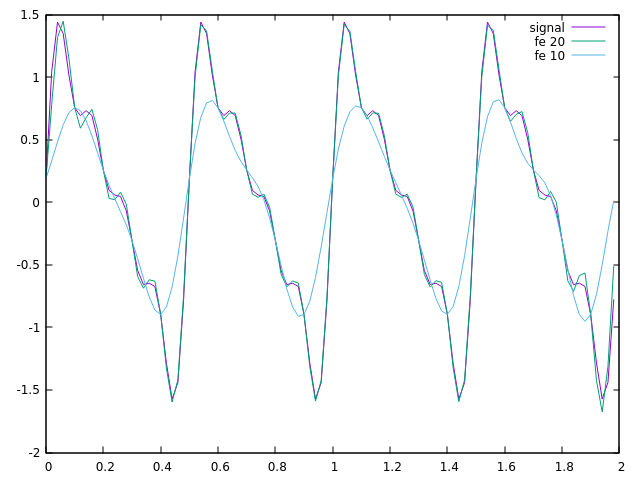
\includegraphics[scale=0.75]{Figures/Result.png}
\end{center}

\end{document}